\documentclass[letterpaper,10pt,conference]{ieeeconf}

\IEEEoverridecommandlockouts
\overrideIEEEmargins

\usepackage{amsmath,amssymb}
\usepackage{flushend}
\usepackage{graphicx}
\usepackage{url}
\usepackage[nocompress]{cite}
% Documented ieeeconf compatibility override: its legacy fake natbib hook
% otherwise disables citation hyperlinks. The official class is unchanged.
\makeatletter
\let\NAT@parse\undefined
\makeatother
\usepackage[hidelinks]{hyperref}

\newtheorem{theorem}{Theorem}
\newtheorem{proposition}{Proposition}
\newtheorem{corollary}{Corollary}
\newtheorem{lemma}{Lemma}
\newcommand{\Post}{\operatorname{Post}}
\newcommand{\cR}{\mathcal R}
\newcommand{\cB}{\mathcal B}

\title{Minimum Output Alphabets for Safe Control\\Under Perception Completion Deadlines}

\author{Fawad Sarim%
\thanks{Fawad Sarim is with the Department of Computer Engineering,
COMSATS University Islamabad, Wah Campus, Wah Cantt 47040, Pakistan, and also with
Pesgit Engineering Services (SMC-Private) Limited, Rawalpindi 46000, Pakistan.
E-mail: mfawadsarim@gmail.com (preferred
correspondence). Telephone: +923399100007.
Mailing address: House no. 1921, Street 32, I-10/2, Islamabad, Pakistan 44000.
\mbox{ORCID: 0009-0002-8997-9288}.}}

\begin{document}
\maketitle

\begin{abstract}
We characterize the coupling between perception output cardinality and computation liveness. For a
finite nondeterministic plant, a static sound partition of the captured state, and a result that may
arrive at any age but is guaranteed by a deadline, we give an exact recursion over propagated
label-conditioned beliefs. For any pending input sequence, the minimum output alphabet equals the
weak chromatic number of the hypergraph of inclusion-minimal captured subsets whose propagation
loses bounded recoverability. Every finite conflict clutter is realizable by a deterministic
one-step-recovery plant. Consequently, complete rank-$r$ conflicts require
$\lceil n/(r-1)\rceil$ symbols although their pairwise conflict graph is empty for \mbox{$r\ge3$}.
Static outputs can require $n$ symbols when an age-dependent output needs only two. Minimizing over
pending sequences yields an exact information--completion frontier whose decision problem is
NP-complete with one-step recovery at every fixed deadline. Three differently structured exact algorithms agree on 972
bounded-exhaustive and 600 five-uncertain-state queries. Conversely, if noncompletion through a safe
watchdog is admissible and outputs are optional, refinement has zero deterministic feasibility
value. A recovery-word Set Cover construction gives a polynomial-time harmonic-factor approximation
at fixed horizons, with an inherited tight logarithmic inapproximability threshold.
\end{abstract}

\section{Introduction}

Neural perception exposes two resources to a controller: information in the returned label and
time at which that label becomes available. Latency--error contract methods select operating points
whose timing is assumed by the controller \cite{pant2015,pant2021,aldana2023}. Anytime-perception
verification instead propagates the states reachable under different update rates
\cite{gupta2024,gupta2025}. Neither an empirical latency percentile nor a fast average execution,
however, is a deterministic completion guarantee.

The neighboring control literature is extensive. Delayed safety games synthesize strategies for
given observation and actuation delays \cite{chen2021}; missing-measurement patterns can be encoded
by automata and reduced to full-information games \cite{yang2021}; and eyes-closed kernels address
permanent loss of observability \cite{laine2020}. Runtime-assurance work preserves recoverability
or a safe backup under perception shift and missed computation deadlines
\cite{sinha2023,nigam2023}. Thus delay, missing data, fallback, and backward safety
synthesis are not individually new contributions.

Information design is equally mature. Action-based sensing derives the information needed by a
control plan \cite{erdmann1995}; plan-lattice methods further relate action choices, memory, and
sensing, including the conversion of compatible-action covers to sensor partitions
\cite{mcfassel2023}. Invariance-feedback entropy uses invariant covers to characterize
data rates for ongoing control \cite{tomar2021}; our objective is a single static label supporting
finite recovery at every allowed completion age, not an asymptotic communication rate.
Sensor predicates can be refined to restore realizability in
partial-information games \cite{fu2014}, while recent invariance work jointly learns a state
partition and a compact control codebook at a fixed sampling period \cite{yuceel2026}. Sensor
activation has also been minimized under control and observation delays \cite{hou2025}.
Liang et al. synthesize supervisors for prescribed delayed event/state observation structures
\cite{liang2024}; here the captured-state alphabet and pending inputs are design variables, and
every admissible completion age must leave bounded open-loop recovery. For constructed filters,
sensor-map minimization is NP-hard and can equal a source graph's chromatic number
\cite{saberifar2019}. Neither coloring nor cover-to-partition conversion alone is new: our distinct object is a plant-induced
higher-order clutter over propagated captured subsets, proved below to realize every finite
clutter even with deterministic one-step recovery.

This letter isolates a narrower question not answered by any one of these formulations: \emph{how
many sound outputs are needed as a function of the contract on when a perception result must
arrive?} Its contributions are:

1) an exact fixed-partition synthesis that propagates captured-state labels through every possible
completion age up to a forced deadline;

2) an exact, partition-independent higher-order conflict hypergraph for the minimum static output
alphabet, jointly optimized with the pending control sequence, and a universality theorem for its
plant-induced structure, plus a recovery-word Set Cover construction giving a polynomial-time
harmonic-factor approximation for fixed recovery and completion horizons;

3) NP-completeness with one-step recovery at every fixed deadline, an unbounded failure of pairwise
reasoning, a sharp product bound and unbounded static-versus-age-dependent gap, and a deadline staircase; and

4) executable agreement among three differently structured exact methods and a no-result boundary that
isolates the role of completion liveness.

All claims are relative to the finite policy class stated below; no general sensor-minimization or
delay-synthesis priority claim is made. AI-assisted drafting is disclosed in the Acknowledgment
\cite{openai2026codex}.

\section{Model and Recovery Primitive}

Let $Z$ be a finite state set, $S\subseteq Z$ the safe states, and $K\subseteq S$ a terminal
recovery set. A nonempty launch belief $X\subseteq S$ contains the physical state. For a finite control
alphabet $U$ and total nondeterministic map $F:Z\times U\to 2^Z\setminus\{\emptyset\}$, define
\begin{equation}
 \Post(X,u)=\bigcup_{x\in X}F(x,u).
\end{equation}
Pending and recovery controls are restricted to nonempty $U_p,U_r\subseteq U$. While a job is
pending, no plant observation is received. The controller nevertheless knows the current belief
from the captured $X$, its applied inputs, and $F$.\footnote{AI-assisted text: \cite{openai2026codex};
see Acknowledgment.}

For recovery horizon $H\in\mathbb N_0$, define
\begin{align}
 \cR_0&=\{X:\emptyset\ne X\subseteq K\},\nonumber\\
 \cR_{h+1}&=\cR_h\cup\{\emptyset\ne X\subseteq S:\nonumber\\
 &\qquad\exists u\in U_r,\ \Post(X,u)\in\cR_h\}. \label{eq:recovery}
\end{align}

\begin{lemma}[Recovery and downward closure]
$X\in\cR_H$ iff one common recovery sequence of length at most $H$ keeps every nondeterministic
image in $S$ and reaches $K$. Moreover, $\cR_H$ is downward closed.
\end{lemma}
\begin{proof}
Induction on $h$ in \eqref{eq:recovery} proves the first statement. If $X'\subseteq X$, then
$\Post(X',u)\subseteq\Post(X,u)$ for every $u$; induction proves the second for nonempty $X'$.
\end{proof}

A job captures belief $X$. Its static sound output map is a partition
$P=\{C_1,\ldots,C_q\}$ of $Z$ whose cells label the captured state. For a pending sequence
$\sigma=(u_0,\ldots,u_{d-1})$, define
$\Phi_{\sigma,0}(A)=A$ and
$\Phi_{\sigma,j+1}(A)=\Post(\Phi_{\sigma,j}(A),u_j)$.
If label $i$ arrives at age $j$, the current-state posterior is therefore
$\Phi_{\sigma,j}(X\cap C_i)$, not $\Phi_{\sigma,j}(X)\cap C_i$.
The controller knows the age and applied inputs, and may use a different recovery sequence for
every posterior. Completion may occur at any age $0,\ldots,d$, for $d\in\mathbb N_0$, and is forced at $d$; until then the
only observation is ``pending.'' Arrival is an irrevocable architecture switch from pending
control to recovery: the controller cannot buffer or decline an early result in this policy class.
Allowing either operation defines a different game. The deterministic resource measured below is
alphabet cardinality $q$; a fixed-length binary interface uses $\lceil\log_2q\rceil$ bits, but no
probability law, entropy, or average-rate objective is assumed.
The contract admits every completion age along every plant trajectory; timing therefore carries
no additional state information. A contract with state-dependent timing support defines a
different observation model. Safety here is through arrival in $K$; indefinite operation after
recovery additionally requires an invariant terminal set and a certified continuation policy.

\section{Fixed-Partition Completion Synthesis}

Discarding empty cells, let $\mathbf Y_P(X)$ be the tuple of captured-cell beliefs
$X\cap C_i$.\footnote{AI-assisted text: \cite{openai2026codex}; see Acknowledgment.}
For a tuple $\mathbf Y=(Y_1,\ldots,Y_\ell)$, define
$T_u\mathbf Y=(\Post(Y_1,u),\ldots,\Post(Y_\ell,u))$ and
\begin{align}
 \mathcal G&=\{\mathbf Y:\emptyset\ne Y_i\subseteq S,\ Y_i\in\cR_H,\ \forall i\},\quad
 \cB_0=\mathcal G,\nonumber\\
 \cB_{d+1}&=\mathcal G\cap
 \{\mathbf Y:\exists u\in U_p,\ T_u\mathbf Y\in\cB_d\}.   \label{eq:layers}
\end{align}

\begin{theorem}[Fixed-partition synthesis]\label{thm:fixed}
\mbox{$\mathbf Y_P(X)\in\cB_d$} iff a deterministic strategy is safe for every completion age
$0,\ldots,d$, with completion forced at $d$, and every propagated label posterior reaches $K$
within $H$ recovery steps.
\end{theorem}
\begin{proof}
At $d=0$, every possible label posterior must lie in $\cR_H$, which is exactly
$\mathbf Y_P(X)\in\mathcal G$. Suppose the claim holds at $d$. At deadline $d+1$, immediate
completion requires $\mathbf Y_P(X)\in\mathcal G$. On the pending branch one common input is
applied, propagating every captured-cell belief to $T_u\mathbf Y_P(X)$, after which precisely the
deadline-$d$ problem remains. This is \eqref{eq:layers}. Concatenating witnesses proves
sufficiency; restricting a winning strategy to its completion and pending branches proves
necessity.
\end{proof}

A noncontiguous advertised age set can instead be represented by an age-indexed recovery gate,
while retaining safe pending propagation between supported ages. We use all ages
$0,\ldots,d$ because that is the completion-by-$d$ contract and yields the monotonicity below.

\begin{proposition}[Monotonicity]
The layers are nested, $\cB_{d+1}\subseteq\cB_d$. If $P'$ refines $P$ and
$\mathbf Y_P(X)\in\cB_d$, then $\mathbf Y_{P'}(X)\in\cB_d$.
\end{proposition}
\begin{proof}
The first inclusion follows by induction from \eqref{eq:layers}. Under refinement, every captured
cell is split into subsets. Their images under any common input sequence remain subsets of the
corresponding coarse-cell images. Downward closure of $\cR_H$ therefore lets the same pending
sequence certify every refined posterior.
\end{proof}

This recursion is useful for a given sensor but remains a standard-looking predecessor operation.
The central question is instead to optimize $P$ and the pending inputs together.

\section{Minimum Information as Hypergraph Coloring}

Write $n=|X|$. Fix a safe pending sequence $\sigma$ of length $d$.\footnote{AI-assisted text:
\cite{openai2026codex}; see Acknowledgment.} Its recovery-conflict hypergraph has captured
vertices $X$ and inclusion-minimal failing subsets
\begin{align}
 \mathcal N_\sigma
   &=\{\emptyset\ne A\subseteq X:\exists j\in\{0,\ldots,d\},\nonumber\\[-1mm]
   &\hspace{31mm}\Phi_{\sigma,j}(A)\notin\cR_H\},\nonumber\\
 E_\sigma&=\min_{\subseteq}\mathcal N_\sigma.                 \label{eq:hypergraph}
\end{align}
A weak coloring forbids every hyperedge from being monochromatic. Write $\chi_w(E_\sigma)$ for
the minimum colors, with value $\infty$ when a singleton edge exists.

\begin{theorem}[Fixed-sequence coloring]\label{thm:coloring}
For a fixed safe sequence $\sigma$, a static sound partition with at most $q$ nonempty cells makes
every completion age recoverable iff \mbox{$\chi_w(E_\sigma)\le q$}.
\end{theorem}
\begin{proof}
Color a state by its partition cell. If an edge $M\in E_\sigma$ were monochromatic, then at the
failing age its image would be contained in one propagated label posterior. If that posterior were
in $\cR_H$, downward closure would put $\Phi_{\sigma,j}(M)$ in $\cR_H$, a contradiction. Thus a
feasible partition is a weak coloring.

Conversely, suppose the propagated posterior of captured cell $A=X\cap C_i$ were nonrecoverable
at some age. Then $A$ is a failing captured subset and, by finiteness, contains an
inclusion-minimal failing $M\in E_\sigma$. It is monochromatic, contradicting weak coloring.
States outside $X$ can be assigned arbitrarily to an existing color.
\end{proof}

Unrolling Theorem~\ref{thm:fixed} searches pending sequences for a fixed $P$, whereas
Theorem~\ref{thm:coloring} searches
partitions for a fixed $\sigma$. Both test the same finite feasible pairs $(P,\sigma)$; hence the
two minimizations commute, and the corollary below performs both.

The hypergraph is partition-independent: it is computed before exact coloring, avoiding direct
Bell-number partition enumeration, although both routes remain exponential. The next result shows
that the higher-order object is not an artifact of a loose abstraction.

\begin{proposition}[Conflict-clutter universality]\label{prop:universality}
For every nonempty finite $X$ and clutter $\mathcal C\subseteq2^X\setminus\{\emptyset\}$ (no member contains
another), there is a deterministic $(|X|+2)$-state plant with $H=1,d=0$ whose minimal recovery
conflicts are exactly $E_{()}=\mathcal C$.
\end{proposition}
\begin{proof}
Add terminal $k$ and unsafe $\bot$, both absorbing. Call $I\subseteq X$ independent when it
contains no member of $\mathcal C$. For every maximal independent $I$, add recovery input $r_I$
that sends $x\in I$ to $k$ and $x\notin I$ to $\bot$. Every nonempty independent subset extends to a
maximal one because $X$ is finite, and hence is one-step recoverable. A dependent subset contains
an edge and no $r_I$ recovers it. Its inclusion-minimal failures are precisely the clutter
members, including singleton infeasibility when present.
\end{proof}
This is a realization result; the family of maximal independent sets, and hence the recovery
alphabet, can be exponential in $|X|$.

\begin{corollary}[Unbounded failure of pairwise reasoning]\label{cor:uniform}
For every $n\ge r\ge3$, a deterministic one-step plant realizes the complete rank-$r$ clutter
$\binom{X}{r}$ and has
\begin{equation}
q^*(X,0)=\left\lceil\frac{n}{r-1}\right\rceil .             \label{eq:uniform}
\end{equation}
Its pairwise conflict graph is empty and therefore predicts one symbol.
\end{corollary}
\begin{proof}
Apply Proposition~\ref{prop:universality}. A weak coloring of $\binom{X}{r}$ has color classes of
size at most $r-1$, giving the lower bound in \eqref{eq:uniform}; grouping vertices into sets of
that size attains it. No two-element edge exists. Thus, already at fixed $r=3$, the true alphabet
$\lceil n/2\rceil$ grows without bound while every pairwise test returns one.
\end{proof}
For $n=r=3$, the three recovery inputs succeed on $\{a,b\}$, $\{a,c\}$, and $\{b,c\}$,
respectively. Every pair has a common safe recovery input, but the triple has none.

Let $\Sigma_d(X)$ contain the length-$d$ pending sequences whose every prefix belief lies in $S$,
and, making the recovery horizon explicit, define
\begin{equation}
 q_H^*(X,d)=\min_{\sigma\in\Sigma_d(X)}\chi_w(E_\sigma),       \label{eq:frontier}
\end{equation}
with the minimum of an empty set defined as $\infty$; the subscript is suppressed when $H$ is fixed.

\begin{corollary}[Exact frontier]
$q^*(X,d)$ is exactly the minimum static output alphabet for which some safe pending strategy
exists under the completion-by-$d$ contract. Moreover, $q^*(X,d)$ is nondecreasing in $d$, treating
$\infty$ as the largest value, while $q_{H+1}^*(X,d)\le q_H^*(X,d)$.
\end{corollary}
\begin{proof}
Before completion, repeated ``pending'' is the only observation, so every deterministic strategy
induces one sequence in $\Sigma_d(X)$. The theorem and minimization prove exactness. A length
$d+1$ witness truncated after $d$ inputs remains a witness, and its conflict hypergraph only loses
failure conditions, proving deadline monotonicity. Finally, $\cR_H\subseteq\cR_{H+1}$, so every
horizon-$H$ witness remains feasible at horizon $H+1$.
\end{proof}

Let $\tau(X,\mathcal C)$ be the minimum number of sets from $\mathcal C$ covering $X$, with
value $\infty$ if no cover exists. The next construction avoids enumerating captured subsets.

\begin{theorem}[Constructive cover at fixed horizons]\label{thm:wordcover}
Put $r=|U_r|$, $p=|U_p|$, and $R=\sum_{h=0}^H r^h$. For each safe $\sigma$, a family
$\mathcal C_\sigma$ of at most $R^{d+1}$ feasible captured sets can be constructed directly from
the transition table, with
$\tau(X,\mathcal C_\sigma)=\chi_w(E_\sigma)$.
When $q^*$ is finite, greedy cover over these families returns a feasible alphabet satisfying
\begin{equation}
 q^*(X,d)\le\widehat q\le \mathrm H_n q^*(X,d),\qquad
 \mathrm H_n=\sum_{i=1}^n\frac1i ,                          \label{eq:greedy}
\end{equation}
in time
$p^d R^{d+1}\operatorname{poly}(|Z|,n,H,d,L)$, where $L$ is the explicit transition-table size.
Thus the approximation is polynomial-time for every fixed $H,d$.
\end{theorem}
\begin{proof}
For every recovery word $\rho$ of length at most $H$, let $W_\rho$ be the safe states from which
the entire word stays safe and ends in $K$. Compute these sets by universal predecessors:
$W_{()}=K$ and
$W_{(u,\rho)}=\{z\in S:F(z,u)\subseteq W_\rho\}$.
For each age and word, compute
$A_{j,\rho}=\{x\in X:\Phi_{\sigma,j}(\{x\})\subseteq W_\rho\}$ by singleton propagation.
Let $\mathcal C_\sigma$ contain the nonempty sets
\begin{equation}
 C(\rho_0,\ldots,\rho_d)=\bigcap_{j=0}^d A_{j,\rho_j}. \label{eq:wordcover}
\end{equation}
Union preservation of $\Phi$ implies that $\rho_j$ recovers the age-$j$ image of each such $C$.
Conversely, any feasible captured cell has one recovery word per age and is contained in the
corresponding intersection. Thus each feasible partition extends to a cover. Conversely, order a
cover and assign each state to its first containing set; downward closure makes the resulting
nonempty cells feasible. This proves equality of optima. Unit-cost greedy Set Cover has factor
$\mathrm H_n$ \cite{chvatal1979}; applying it to an optimal pending sequence and retaining the
best result over all sequences proves \eqref{eq:greedy}. There are $R^{d+1}$ word tuples and at
most $p^d$ pending sequences. All predecessors, singleton images, intersections, and greedy steps
take polynomial work per tuple (at most $n$ sets are selected). No uniform polynomial bound in
$H,d$ is claimed.
\end{proof}

Both interfaces below reveal arrival age to the controller. An age-dependent encoder may use a
different captured-state partition $P_j$ at each age; the static encoder must use one $P$.

\begin{proposition}[Sharp age-product bound]\label{prop:product}
Fix a safe $\sigma$ and let $q_j$ be the minimum captured-state alphabet needed for recovery only
at age $j$. If all $q_j$ are finite, then
\begin{equation}
 \max_j q_j\le\chi_w(E_\sigma)\le
 \min\left\{n,\prod_{j=0}^d q_j\right\}. \label{eq:product}
\end{equation}
For any positive integers $q_0,\ldots,q_d$, the product bound is attained by a deterministic
plant with $H=1$, $N=\prod_jq_j$ captured states, $(d+1)N+2$ total states, and
$1+\sum_jq_j$ inputs.
\end{proposition}
\begin{proof}
An all-age partition works at each individual age, proving the lower bound. Intersect optimal
age-wise partitions; their nonempty intersections are feasible by downward closure and number at
most $n$ and $\prod_jq_j$. For equality, capture vectors
$v\in\prod_{j=0}^d\{1,\ldots,q_j\}$. Create safe layered states $x_{j,v}$ and absorbing
terminal $k$ and unsafe $\bot$, with $X=\{x_{0,v}\}$. The sole pending input advances layers, saturating at $d$.
Recovery input $r_{j,a}$ sends $x_{j,v}$ to $k$ iff $v_j=a$, and every other layered state to
$\bot$. At age $j$, exactly $q_j$ coordinate classes are needed. Any two distinct captured
vectors differ at some age's coordinate, so they cannot share a static cell; hence $N$ are
necessary and sufficient.
\end{proof}

\begin{proposition}[Unbounded static-interface cost]\label{prop:staticgap}
For every $n\ge2$, there is a deterministic plant with $H=1$ and one pending input for which a
static captured-state output requires $n$ symbols, whereas an age-dependent output requires
exactly two at every possible completion age.
\end{proposition}
\begin{proof}
Decompose the edges of $K_n$ into nonempty matchings $M_0,\ldots,M_{m-1}$ by the round-robin
construction, where $m=n-1$ for even $n$ and $m=n$ for odd $n$ (add and then delete a dummy
vertex). Set $d=m-1$. Create states $x_{j,v}$ for every layer $j$ and vertex $v$, plus absorbing $k$ and
$\bot$. The pending input advances $x_{j,v}$ to $x_{\min\{j+1,m-1\},v}$. At layer $j$, use the
construction of Proposition~\ref{prop:universality} for clutter $M_j$, with its recovery inputs
unsafe on all other layers. Thus the captured pair conflicts at age $j$ are exactly $M_j$.
Their union over completion ages $0,\ldots,m-1$ is $K_n$, so a static coloring needs $n$ symbols.
At a known age, the nonempty matching $M_j$ is bipartite and needs exactly two; its two color
classes are recoverable by the construction.
\end{proof}
Thus the static interface is a substantive restriction, not without loss of generality; changing
it also changes which age-indexed output maps a perception implementation must realize.

\begin{figure*}[t]
\centering
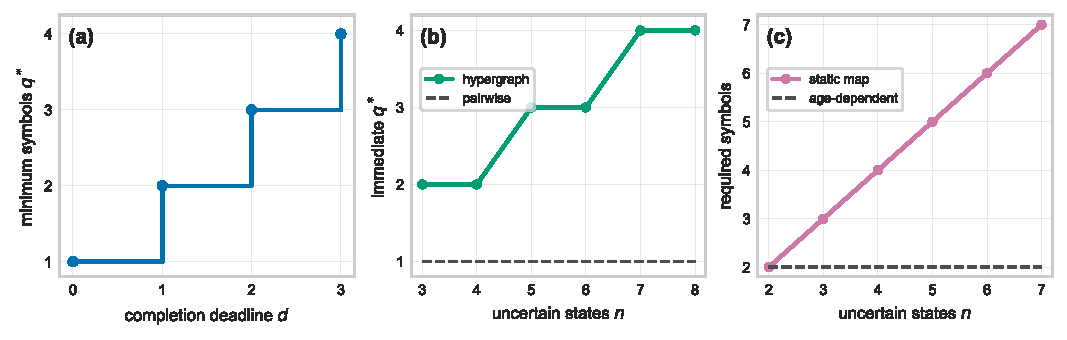
\includegraphics[width=0.98\textwidth]{figures/information_completion.pdf}
\caption{Exact information--completion frontiers. (a) A construction whose minimum alphabet grows
with the deadline. (b) Complete ternary conflicts require $\lceil n/2\rceil$ symbols while their
pairwise conflict graph reports one.
(c) Static captured-state outputs require $n$ symbols while age-dependent outputs require two.}
\label{fig:frontier}
\end{figure*}

\subsection{Complexity and tight families}

Let $n=|X|$ and $p=|U_p|$. After $\cR_H$ membership is available, direct frontier enumeration
uses at most $p^d(d+1)(2^n-1)$ recovery-membership queries and one exact weak-coloring call per safe
pending sequence. If $T_\chi(n,m)$ denotes that coloring cost, the oracle work is
$O\!\left(p^d[(d+1)2^n+T_\chi(n,2^n-1)]\right)$, apart from belief propagation. A cheap lower
certificate uses the graph on $X$ joining $x,y$ when
$\{x,y\}\notin\cR_H$: any exhibited clique $Q$ certifies $q_H^*(X,d)\ge |Q|$, since completion may
occur at age zero. A nonrecoverable singleton certifies infeasibility.
Corollary~\ref{cor:uniform} shows that this pairwise bound can remain one while the optimum diverges.

\begin{theorem}[Complexity at $d=0$]\label{thm:hardness}
With $H=1$ and \mbox{$d=0$}, deciding $q^*(X,0)\le q$ is NP-complete for deterministic plants.
\end{theorem}
\begin{proof}
Under explicit transition-table encoding, membership in NP follows by guessing a partition and zero or one recovery input per posterior, then
checking all explicit transitions. For hardness, reduce Set Cover \cite{karp1972}. Given universe
$V$, sets $A_1,\ldots,A_m$, and budget $q$, create safe states $V\cup\{k\}$, absorbing unsafe state
$\bot$, and $K=\{k\}$. Input $u_i$ sends $v$ to $k$ iff $v\in A_i$, and to $\bot$ otherwise; $k$
and $\bot$ are absorbing. With initial belief $V$, a posterior is one-step recoverable iff it is
contained in some $A_i$. Hence at most $q$ feasible cells imply a set cover of size at most $q$.
Conversely, assign each element to one selected set containing it; the nonempty assignments form a
feasible partition. The construction is polynomial.
\end{proof}

\begin{corollary}[Hardness at every fixed deadline]
For every fixed $d\ge0$, deciding $q^*(X,d)\le q$ remains NP-complete with $H=1$ and
deterministic plants, even with a singleton pending alphabet.
\end{corollary}
\begin{proof}
Membership is certified by a partition, the fixed-length pending sequence, and zero or one recovery input
per cell and completion age. For hardness, add one safe pending input that self-loops every state in
the Set Cover construction. Every age then has the same posteriors, so
$q^*(X,d)=q^*(X,0)$.
\end{proof}

\begin{corollary}[Logarithmic inapproximability]\label{cor:inapprox}
For every constant $0<\alpha<1$ and fixed $d\ge0$, it is NP-hard to approximate finite
$q^*(X,d)$ within $(1-\alpha)\ln n$, even for deterministic plants, $H=1$, and a singleton
pending alphabet.
\end{corollary}
\begin{proof}
The reduction above preserves exactly the Set Cover universe size $n$ and optimum, and the
self-loop padding preserves both for any fixed $d$. The claim follows from the tight Set Cover
threshold \cite{dinur2014}.
\end{proof}

\begin{proposition}[Exact deadline staircase]
For every \mbox{$D\ge0$}, a $((D+1)^2+2)$-state, $(D+2)$-input deterministic plant with $H=1$ satisfies
$q^*(X,d)=d+1$ for all $0\le d\le D$.
\end{proposition}
\begin{proof}
Reuse terminal state $k$ and unsafe absorbing state $\bot$. Use branches
$b\in\{0,\ldots,D\}$, layers $j\in\{0,\ldots,D\}$, and states $x_{j,b}$. The sole pending input
maps $x_{j,b}$ to $x_{\min\{j+1,D\},b}$. At layer $j$, recovery input $r_i$ reaches $k$ exactly
when $i=\min\{b,j\}$; all other recovery inputs reach $\bot$. Unmentioned transitions are
absorbing. Start from
$X=\{x_{0,b}:0\le b\le D\}$. At age $d$, captured branches
$0,\ldots,d-1$ and the tail $d,\ldots,D$ require $d+1$ distinct recovery inputs, so they cannot
share output cells. Conversely, label captured branch $b$ by $\min\{b,d\}$. At every earlier age
$j\le d$, branches sharing a label also share recovery input $r_{\min\{b,j\}}$. Thus $d+1$
symbols are both necessary and sufficient.
\end{proof}

\noindent\textit{Boundary (optional outputs).}
If noncompletion through a finite watchdog is admissible, each output may be ignored, fallback
resources do not block, and late outputs have no authority, refinement has zero deterministic
feasibility value. Necessity follows by restricting any winning strategy to the admissible
no-result execution; sufficiency follows by ignoring outputs. This elementary boundary neither
denies performance value nor safety gains under guaranteed completion; it isolates why the
liveness premise in \eqref{eq:frontier}, not measured accuracy alone, enables the frontier.

\section{Exact Computational Checks}

Three deliberately different finite solvers implement (i) the tuple recursion \eqref{eq:layers},
(ii) pending-sequence enumeration and exact hypergraph coloring, and (iii) canonical sensor-map,
pending-sequence, and recovery-sequence enumeration. The third does not call either production
solver.\footnote{Code: \url{https://github.com/fawadsarim/safe-control-output-alphabets}.
AI-assisted text: \cite{openai2026codex}; see Acknowledgment.}
Tests distinguish captured-state propagation from the incorrect completion-state
intersection and cover the boundary cases and parametric families. The bounded class exhausts two
safe states plus one absorbing unsafe state, two deterministic controls, $K=\{0\}$, $H=1$, all
$3^4=81$ transition tables, three nonempty launch beliefs, and four deadlines: all 972 queries
agree. With seed 20260904, a further 600 five-uncertain-state nondeterministic queries agree.
Separately, 20 nondeterministic plants, up to four partitions, and three deadlines compare the
fixed-partition recursion with exhaustive sequence evaluation. Tests also exhaust all 19 clutters
on three vertices and reproduce Corollary~\ref{cor:uniform} through $n=8$ and
Proposition~\ref{prop:staticgap} through $n=7$; the cover dual and greedy certificate are checked
on all 167 clutters over four vertices. The recovery-word construction is checked separately on
216 queries (24 nondeterministic plants, $H,d\in\{0,1,2\}$): its exact cover optimum agrees with
canonical-map enumeration, and every returned greedy cell carries directly checked recovery words
for all ages. Of these 216 queries, 205 are infeasible. A separate constructed family supplies
72 feasible queries (12 state relabelings, $H\in\{1,2\}$, $d\in\{0,1,2\}$), all with optimum two.
With self-loop pending control, greedy needs three cells; allowing a nondeterministic switch
attains two for $d\ge1$. Direct transition checks verify every witness and reject unsafe pending
sequences. At $H=d=1$, a six-state constructed plant needs two labels under a separating pending
input but only one when a merging input is allowed; direct witnesses certify both optima.
Ten coordinate constructions check \eqref{eq:product} at every prefix and age.
These are executable equivalence and construction checks, not statistical claims.

Figure~\ref{fig:frontier} reproduces the frozen deadline staircase, higher-order conflicts, and
static-interface separation. Randomized queries check algorithm agreement, not physical frequencies.

\section{Limitations and Conclusion}

Exact partition and coloring search is exponential; the polynomial approximation holds only for
fixed horizons. The model assumes a finite abstraction, static
sound captured-state outputs (shown above to be more restrictive than age-dependent maps), finite
alphabets and horizons, no plant observation while pending, an irrevocable completion switch, and
posterior-specific open-loop recovery only after completion. A classifier must separately
implement the sound partition; a scheduling or verification argument must separately establish
forced completion by $d$, which a measured latency percentile cannot do. No device, energy,
flight, neural-network, or physical-frequency claim follows from the executable audits.

Within these limits, the result makes the timing assumption behind information-dependent safety
explicit and computable. Guaranteed completion yields an exact recovery-conflict coloring problem;
admissible noncompletion collapses optional output information out of deterministic feasibility.
This frontier is the practical distinction between measuring that a perception mode is usually
fast and proving that its information can be used in a hard-safety argument.

\noindent\textit{AI-assisted text:} \cite{openai2026codex}; see Acknowledgment.

\section*{Acknowledgment}
OpenAI Codex assisted with manuscript drafting and editing throughout the paper, code
development, and drafting and inspecting proof arguments. The author takes sole responsibility
for the scientific content, analyses, references, and conclusions.

\bibliographystyle{IEEEtran}
% Balance at an entry boundary using the class's supported hook. Automatic
% balancing stretches hyperlink-bearing bibliography entries unevenly.
\raggedend
\raggedbottom
\interlinepenalty=10000\relax
\IEEEtriggercmd{\newpage}
\IEEEtriggeratref{11}
\bibliography{references}

\end{document}
